%!TEX TS-program = xelatex
%!TEX options = -aux-directory=Debug -shell-escape -file-line-error -interaction=nonstopmode -halt-on-error -synctex=1 "%DOC%"
\documentclass{article}
\input{LaTeX-Submodule/template.tex}

% Additional packages & macros

% Header and footer
\newcommand{\unitName}{Embedded Systems}
\newcommand{\unitTime}{Semester 1, 2025}
\newcommand{\unitCoordinator}{Dr Chris Lehnert}
\newcommand{\documentAuthors}{Tarang Janawalkar}

\fancyhead[L]{\unitName}
\fancyhead[R]{\leftmark}
\fancyfoot[C]{\thepage}

% Copyright
\usepackage[
    type={CC},
    modifier={by-nc-sa},
    version={4.0},
    imagewidth={5em},
    hyphenation={raggedright}
]{doclicense}

\date{}

\begin{document}
%
\begin{titlepage}
    \vspace*{\fill}
    \begin{center}
        \LARGE{\textbf{\unitName}} \\[0.1in]
        \normalsize{\unitTime} \\[0.2in]
        \normalsize\textit{\unitCoordinator} \\[0.2in]
        \documentAuthors
    \end{center}
    \vspace*{\fill}
    \doclicenseThis
    \thispagestyle{empty}
\end{titlepage}
\newpage
%
\tableofcontents
\newpage
%
\section{Introduction}
\subsection{Definition of an Embedded System}
An embedded system is a combination of computer hardware and software
designed for a specific function or functions within a larger system.
These systems typically contain computer hardware \textit{within} their
implementation and are used in devices to simplify system design and
provide flexibility. Often, the user is unaware that a processor is
present in the device as an embedded system comprises a suite of
different components that communicate with each other to perform a
specific task. These components include the processor, memory, and
analog/digital ports---which form the microcontroller---and ports that
are connected to various input/output devices such as sensors,
actuators, and user interfaces---each of which interact with the
environment. This is illustrated in the figure below, where the grey
box represents the embedded system.
\begin{figure}[H]
    \centering
    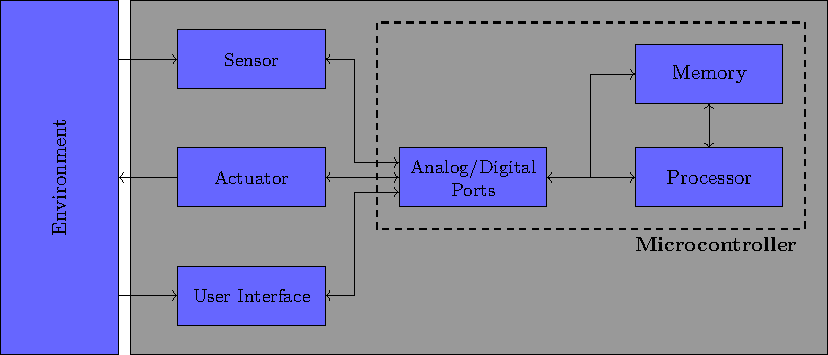
\includegraphics[width = \linewidth]{figures/embedded_system_structure.pdf}
    % \caption{} % \label{}
\end{figure}
\subsubsection{Types of Embedded Systems}
Embedded systems can be classified into three main categories:
\begin{itemize}
    \item \textbf{Centralised:} One node performs all work.
    \item \textbf{Distributed:} Nodes distribute work across sub-nodes.
    \item \textbf{Decentralised:} Nodes are only connected to peers in a network.
\end{itemize}
\subsection{Advanced RISC Machines}
Advanced RISC Machine (ARM) is a family of Instruction Set
Architectures (ISAs) for computer processors. These ISAs are developed
and designed by Arm Holdings so that they can be licensed to other
companies that design their own ARM-based processors. ARM processors
are found in many battery operated devices such as mobile phones,
tablets, embedded systems, and some newer laptops.

Reduced Instruction Set Computer (RISC) processors are popular in such
applications due to their high performance per watt and ability to
execute all instructions in a single cycle. Additionally, because the
architecture uses fixed-length instructions, instructions are also
easier to pipeline, leading to increased parallelism. The RISC
architecture focuses on small and highly-optimised instructions rather
than the highly-specialised set of instructions found on Complex
Instruction Set Computer (CISC) architectures such as x86. Although
this may seem restrictive, this allows instructions to be executed at a
greater frequency resulting in improved performance. Complex operations
can then be performed in software using these instructions.
\subsubsection{ARM Cortex Cores}
ARM develops many families of processing cores for a range of different
functions:
\begin{itemize}
    \item \textbf{Cortex-A}: Highest performance cores---optimised for rich operating systems.
    \item \textbf{Cortex-R}: Fast response cores---optimised for high-performance, hard real-time applications.
    \item \textbf{Cortex-M}: High efficiency cores---optimised for discrete processing and microcontrollers.
    \item \textbf{SecurCore}: Tamper resistant cores---optimised for security applications.
\end{itemize}
\subsection{Characteristics of an Embedded System}
Embedded systems are characterised by several features. At a high
level, they may be designed to be:
\begin{itemize}
    \item Highly stable
    \item Time specific
    \item Task specific
    \item Cost effective
    \item Minimal in interface
    \item Easy to operate
    \item Real-time
    \item High-efficiency
    \item Reliable
    \item Memory constrained
    \item Power constrained
    \item Fault tolerant
\end{itemize}
\subsubsection{Design Goals}
These characteristics lead to several design goals in embedded systems
such as:
\begin{itemize}
    \item Reliability: Some systems may be critical to a mission, or
          life-threatening, and must be able to operate 24/7 without
          rebooting.
    \item Performance: Systems may need to respond to many events
          within a time frame using resources such as computing speed
          and power effectively. Constraints may need to be placed on
          inputs to prevent buffer overflows, and inaccuracies from
          floating-point calculations must be properly handled.
    \item Cost: Systems may be marketed to consumers and must therefore
          manufacturing minimise cost and be easy to produce.
\end{itemize}
\subsection{Real-Time Applications}
A system is said to be real-time if the total correctness of an
operation not only depends on its logical correctness, but also upon
the time in which it is performed. A primary design goal of real-time
systems is \textbf{meeting deadlines}.
\begin{itemize}
    \item \textbf{Soft real-time systems} execute as fast as possible requiring
          on explicit deadline on the response time.
    \item \textbf{Hard real-time systems} impose a strict deadline on the
          response time. If the deadline is missed, the system fails.
\end{itemize}
\subsubsection{Real-Time Operating Systems}
Embedded systems are typically developed using low-level programming
languages such as C, C++, and assembly, for their performance and
reliable compilation. The compilation process is different from that of
a desktop application where code is compiled into an executable file
which can be executed by the operating system. Instead, embedded
systems (or those with sufficient resources) make use of
\textbf{real-time kernel} libraries alongside application code to
produce a single binary image that is flashed onto the device. These
systems are known as real-time operating systems (RTOS). The kernel is
software that manages this real-time system by providing abstractions
for creating threads (tasks), scheduling, input/output operations,
memory management, and other functions in an operating system.
\subsection{Tiva C Series Microcontrollers}
This unit uses the Texas Instruments Tiva C series TM4C1294NCPDT
microcontroller which is housed on the EK-TM4C1294XL evaluation board.
This microcontroller chip is based on an ARM Cortex-M4 core and
includes several on-chip peripherals such as an Ethernet controller,
USB interface, analog-to-digital converters (ADCs), and timers. The
evaluation board also provides additional hardware such as LEDs,
switches, a touch screen, and other input/output devices, all of which
can be interfaced with the microcontroller.
\subsubsection{Arm Cortex-M4 Processor}
Some technical specifications of the Cortex-M4 processor are described
below:
\begin{itemize}
    \item \textbf{Architecture}: Armv7E-M
    \item \textbf{Bus Interface}: 3x Advanced Microcontroller Bus Architecture 3 Advanced High-performance Bus-Lite (AHBA 3 AHB-Lite) interface (Harvard bus architecture)
    \item \textbf{Instruction Set Architecture Support}: Thumb or Thumb-2\footnote{The
              thumb instruction set is a subset of the most commonly used 32-bit ARM
              instructions. Thumb instructions are 16 bits long and have
              corresponding 32-bit ARM instructions that perform the same
              function. They are used to reduce code size and improve
              performance in memory-constrained applications. Thumb2 provides
              enhancements to Thumb by introducing a new conditional instruction
              amongst other improvements.}, hardware divide, single-cycle multiply, etc.
    \item \textbf{Pipeline}: 3-stage (Fetch-Decode-Execute)
\end{itemize}
A block diagram of the Cortex-M4 processor, and its register set are
shown below.
\begin{figure}[H]
    \centering
    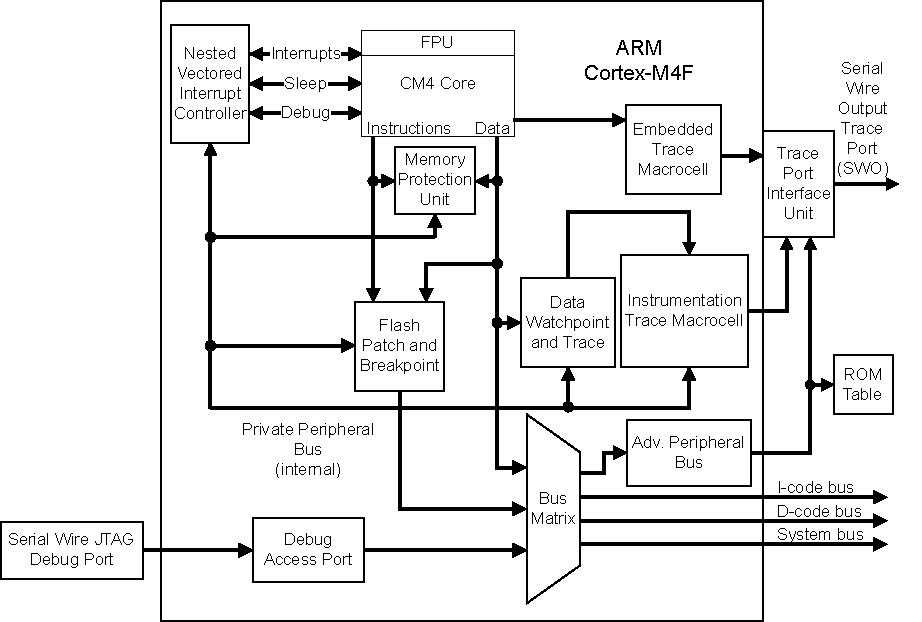
\includegraphics[width = \linewidth]{figures/cortex_m4_block_diagram.pdf}
    \caption{Block diagram of the Cortex-M4 processor.}
\end{figure}
\begin{figure}[H]
    \centering
    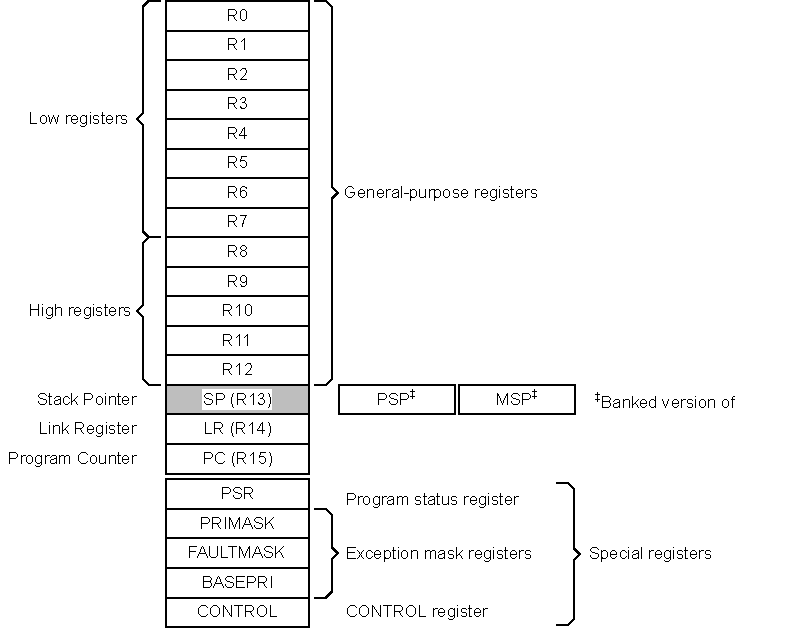
\includegraphics[width = \linewidth]{figures/cortex_m4_register_set.pdf}
    \caption{Register set of the Cortex-M4 processor.}
\end{figure}
\subsubsection{Programming Models}
Tiva C series microcontrollers can be programmed using the
\textbf{Direct Register Access Model} where the application accesses
hardware registers directly using pointers and bitwise operations. This
model results in small and more efficient code.

The registers in this model can be accessed by including the
\texttt{tm4c1294ncpdt.h} header file, which contains register
definitions for all peripherals on the Tiva C series microcontroller.
\begin{minted}{c}
#include "inc/tm4c1294ncpdt.h"
\end{minted}
The macros in this header file use the following naming conventions:
\begin{itemize}
    \item \textbf{Suffixes}:
          \begin{itemize}
              \item \mintinline{c}{_R}: Access to the memory-mapped register.
              \item \mintinline{c}{_M}: Mask for a multi-bit field.
              \item \mintinline{c}{_S}: Shift value for field alignment.
          \end{itemize}
    \item \textbf{Register Name Structure}: \mintinline{c}{<MODULE><INSTANCE>_<REGISTER>_R}
    \item \textbf{Bit Field Name Structure}: \mintinline{c}{<MODULE><INSTANCE>_<REGISTER>_<FIELD>}. Bit fields
          with multiple values are often suffixed with \mintinline{c}{_M}, \mintinline{c}{_S}, or a value.
\end{itemize}
Alternatively, we can use the \textbf{Software Driver Model} where the
application uses a development API such as the \textbf{TivaWare}
software development kit (SDK) to access hardware registers. This model
aims to simplify the development process by providing functions for
accessing peripherals such as GPIO, UART, I2C, SPI, and ADC.
\subsection{Microcontroller Architecture}
A microcontroller is made up of a microprocessor, memory, peripherals,
and I/O. Communication between the microprocessor and these devices is
facilitated through the system bus that consists of an address bus,
data bus, and control bus\footnote{A bus refers to a group of lines
carrying digital signals.}. This bus allows shared communication
between a single processor and device at a time. To overcome this
limitation and allow multiple devices to communicate with multiple
processors concurrently, a bus matrix is often used instead of, or in
addition to, the system bus. Furthermore, microprocessor architecture
also determines whether code memory and data memory are accessed via
the same data bus, where:
\begin{itemize}
    \item \textbf{von Neumann Bus Architecture} accesses code and data memory from the same bus.
    \item \textbf{Harvard Bus Architecture} accesses code and data memory from two separate buses, called the instruction code bus (I-code bus) and the data code bus (D-code bus).
\end{itemize}
\subsection{Microcontroller Memory}
The TM4C1294NCPDT microcontroller is integrated with the following set
of on-chip memory:
\begin{itemize}
    \item \textbf{Non-Volatile Memory} (retains data when powered off):
          \begin{itemize}
              \item \qty{1024}{K.B} \textbf{Flash Memory} (\(4 \times \qty{256}{K.B}\) banks) used for storing program code.
              \item \qty{6}{K.B} \textbf{Electronically Erasable Programmable Read-Only Memory (EEPROM)} used for storing non-volatile data.
              \item \textbf{Internal Read-Only Memory (ROM)} loaded with
                    TivaWare for C Series software: TivaWare Peripheral
                    Driver Library and TivaWare Boot Loader.
          \end{itemize}
    \item \textbf{Volatile Memory} (loses data when powered off):
          \begin{itemize}
              \item \qty{256}{K.B} \textbf{Single-Cycle Static Random Access Memory (SRAM)} used for very fast data access and frequent
                    read/write operations. This memory is the runtime memory for the
                    program stack, peripheral registers, and runtime variables.
          \end{itemize}
\end{itemize}
\subsubsection{Memory Map}
Desktop architectures typically have separate address spaces for memory
and peripherals, where input and output devices are mapped to a
separate address space. However, the TM4C1294NCPDT microcontroller uses
a shared address space for memory and peripherals, which is known as
the \textbf{memory map}.
\begin{table}[H]
    \centering
    \begin{tabular}{llp{5cm}}
        \toprule
        \textbf{Address Range}                       & \textbf{Memory Region} & \textbf{Description}                                                                                                      \\
        \midrule
        \mintinline{rust}{0x0000_0000 - 0x1FFF_FFFF} & Code                   & This executable region is for program code. Data can also be stored here.                                                 \\
        \mintinline{rust}{0x2000_0000 - 0x3FFF_FFFF} & SRAM                   & This executable region is for data. Code can also be stored here. This region includes bit band and bit band alias areas. \\
        \mintinline{rust}{0x4000_0000 - 0x5FFF_FFFF} & Peripheral             & This region includes bit band and bit band alias areas.                                                                   \\
        \mintinline{rust}{0x6000_0000 - 0x9FFF_FFFF} & External RAM           & This executable region is for data.                                                                                       \\
        \mintinline{rust}{0xA000_0000 - 0xDFFF_FFFF} & External device        & This region is for external device memory.                                                                                \\
        \mintinline{rust}{0xE000_0000 - 0xE00F_FFFF} & Private peripheral bus & This region includes the NVIC, system timer, and system control block.                                                    \\
        \mintinline{rust}{0xE010_0000 - 0xFFFF_FFFF} & Reserved               & -                                                                                                                         \\
        \bottomrule
    \end{tabular}
    \caption{Memory Access Map on the TM4C1294NCPDT Microcontroller.}
\end{table}
\subsubsection{Bit-Banding}
The ARM Cortex-M4 processor supports a feature called
\textbf{bit-banding} which maps a full word of memory to a single bit
in the bit-band region. This eliminates the need for read-modify-write
operations, as individual bits can be set, cleared, or toggled directly
from an alias address. This technique is used on the TM4C1294NCPDT as
it uses a 32-bit word size, resulting in \qty{4}{G.B} of addressable
memory, of which, peripherals only use a small portion. The remaining
region of memory is therefore used for alias addresses that serve this
purpose.
\part{Microcontroller Peripherals}
The following sections highlight the functionality of various
peripherals and provide examples of their configuration using the
TivaWare Peripheral Driver Library.
\section{System Control}
System control determines the overall operation of the device by:
\begin{itemize}
    \item controlling the system clock,
    \item configuring which peripherals are enabled,
    \item configuring the device and its resets, and by
    \item providing information about the device.
\end{itemize}
\subsection{System Clock}
The main system clock is used to clock the processor and all
peripherals on the device. The system clock frequency is determined
through the following steps:
\begin{enumerate}
    \item \textbf{Select the input source:}

          Choose an oscillator source (internal oscillator or external
          crystal) and configure the frequency of the oscillator.
    \item \textbf{Apply a frequency multiplier:} (optional)

          A Phase-Locked Loop (PLL) can be used to multiply an input
          frequency using a Voltage Controlled Oscillator (VCO).
    \item \textbf{Apply Frequency Divider:} (optional)

          The system clock divider can be used to divide the output
          frequency of the PLL or oscillator source.
    \item \textbf{Select the system clock source:}

          Choose whether the system clock is driven by the PLL output
          or directly by the oscillator source.
\end{enumerate}
\subsubsection{Oscillator Source}
The oscillator source can be one of the following:
\begin{itemize}
    \item \mintinline{c}{SYSCTL_OSC_MAIN} to use an external crystal or oscillator.
    \item \mintinline{c}{SYSCTL_OSC_INT} to use the \qty{16}{M.Hz} precision internal oscillator.
    \item \mintinline{c}{SYSCTL_OSC_INT30} to use the internal low frequency oscillator.
    \item \mintinline{c}{SYSCTL_OSC_EXT32} to use the hibernate modules \qty{32.786}{k.Hz} oscillator.
\end{itemize}
When using an external crystal, the frequency is set using the
macro \mintinline{c}{SYSCTL_XTAL_<frequency>MHZ} where
\mintinline{c}{<frequency>} is the frequency of the crystal in \unit{M.Hz}.
\subsubsection{System Clock Source}
The system clock source may be configured to use the output of the PLL
or be directly driven by the oscillator source using one of the
following macros:
\begin{itemize}
    \item \mintinline{c}{SYSCTL_USE_PLL} is used to select the PLL output as the system clock.
    \item \mintinline{c}{SYSCTL_USE_OSC} is used to choose one of the oscillators as the system clock.
\end{itemize}
When using the PLL, the VCO frequency can be configured using one of the
following macros:
\begin{itemize}
    \item \mintinline{c}{SYSCTL_CFG_VCO_480} to set the PLL VCO output to \qty{480}{M.Hz}
    \item \mintinline{c}{SYSCTL_CFG_VCO_320} to set the PLL VCO output to \qty{320}{M.Hz}
\end{itemize}
The \mintinline{c}{SysCtlClockFreqSet()} function attempts to match the
requested system clock frequency to the closest possible value based on
the configuration of the device clocking.
\subsubsection{SysCtlClockFreqSet()}
\textbf{Prototype:}
\begin{minted}{c}
uint32_t SysCtlClockFreqSet(uint32_t ui32Config, uint32_t ui32SysClock);
\end{minted}
\textbf{Parameters:}
\begin{itemize}
    \item \mintinline{c}{ui32Config} is the required configuration of the device clocking.
    \item \mintinline{c}{ui32SysClock} is the requested processor frequency.
\end{itemize}
\textbf{Returns:}
\medskip

The actual configured system clock frequency in Hz or zero if the value
could not be changed due to a parameter error or PLL lock failure.
\subsubsection{Example}
\begin{minted}{c}
#include "inc/tm4c1294ncpdt.h"

int main(void) {
    // Use a 25 MHz external crystal oscillator with a PLL VCO output of
    // 480 MHz.
    // The desired system clock frequency is 120 MHz which will require
    // a system clock divider of 4.
    SysCtlClockFreqSet(SYSCTL_XTAL_25MHZ | SYSCTL_OSC_MAIN |
                       SYSCTL_USE_PLL | SYSCTL_CFG_VCO_480, 120000000);

    // ...
}
\end{minted}

\end{document}
